\chapter{Step Size Adaptation}
\label{ch: stepsize_adaptation}

\graphicspath{{Figures/Stepsize_adapt/}{./}} 

Step size is a key factor in convergence performance. The importance of step size selection is not only shown in our practical experiment results (chapter~\ref{ch: sgd_exp}), but has also been proved in theories of the machine learning ares. Generally in SGD, a large  step size is likely to reach the convergence early in the estimation with a big fluctuation rate. In contrast, a small step size can avoid the big fluctuation after it eventually reach the convergence, which possibility never comes in our quantile estimation problem because the data stream might stop before it converges.
Due to the fact that a small step size for condition might be a big one for another, we want to choose step sizes based on different measurements and heuristics. That is, we want to explore the topic of step size adaptation. 

In this chapter, we conduct the investigation of step size adaptation for SGD quantile estimation. Specifically, we look into two potential machine learning methods on step size adaptation, make analysis and implement one of them on SGD. In addition, we propose another step size adaptation algorithm, and compare the difference between their empirical performances. The contents of this chapther is listed as follows:

Section~\ref{sec: newton} briefly introduces the potential step size adaptation method in machine learning, and explains why it cannot be applied for the SGD algorithm.

Section~\ref{sec: sag} analyses another machine learning method \textit{SAG}, implements it to SGD and conducts experiments to check the convergence performance

Section~\ref{sec: DH_SGD} shows a proposal of another step size adaptation algorithm \textit{DB-SGD}, which is also provided with explanations and empirical experiments.

Section~\ref{sec: stepsize_adaptation_conclusion} compares the two proposed algorithms and discusses about their improvements on convergence.

\section{Failure on Newton's Method}
\label{sec: newton}
Newton's method is an iterative method to find the stationary points (where the function's derivative is zero) of a twice-differentiable function $f$. The application of Newton's method failed for our SGD quantile methods, since the loss function of the quantile estimation function is not twice-differentiable. For a specific $\tau$, and $t := x - q$ be the difference between the input data value $x$ and the estimate of quantile $q$, the loss function 

\begin{equation}
    \ell_\tau(t)= 
        \begin{cases}
            \tau t & t > 0\\
            -(1-\tau) t & otherwise
        \end{cases}
\end{equation}


is a linear function of $t$, which doesn't have any second derivative. 
\\\\
Though the method cannot be applied, it is easy to reach the goal of Newton's method: to find the critical points of a function. Instead of stationary point, the loss function has a critical point where it is not differentiable and the derivative changes sign. For any $\tau \in (0,1)$, when $t=0$, the loss function reaches it's critical points at $\ell_\tau(0) = 0$. Taking the critical point for every step, however, does not contribute to any improvement in quantile estimation. To be at a critical point, the quantile estimate is set to have the equal value of input data $x$, and only in this way we could have $t = x-q = x-x = 0$. Regardless of $\tau$, the quantile estimate is always equal to the value of the latest data point. So far this method has totally failed its goal to estimate a quantile value based on $\tau$ and the entire data stream.
\\\\
From another perspective, the failure of Newton's method is the result of applying large step size for the last input data for a SGD method. In this way, the minimal of current loss function $\ell_\tau(t)$ is reached, while the total loss function for the input data stream $X$

\begin{equation}
    L_{\tau}(t) = \sum_{x \in X} \ell_{\tau}(t)
\end{equation}

is entirely ignored.

% ------------------------------------------------

\graphicspath{{Figures/Smooth_func/}{./}} 


\section{Stochastic Average Gradient (SAG)}
\label{sec: sag}
One approach on step size adaptation is to use the stochastic average gradient (SAG)\cite{schmidtMinimizingFiniteSums2016} algorithm. It is an convex optimization method that has a significant improvement of convergence rate than stochastic gradient (SG) methods. In general, the convergence rate is improved from $O(1/\sqrt{k})$ to $O(1/k)$ for a total of $k$ epochs, reaching the same level as the gradient descent method. Along with the rising convergence rate, it keeps a low computational cost for each iteration to be independent from the size of function sum.

\subsection{Mechanism of SAG}
Recall the update function of SGD (equation~\ref{eq: intro_SGD}), the stochastic average gradient (SAG) remembers the last update of a gradient value for each index $i$, which enables the improvement of convergence rate from SG methods. Its iteration takes the form
\begin{equation}
x_{i+1} = x_i - \frac{\alpha_i}{N} \sum^N_{n=1}y_{m}^{i}
\end{equation}
where $y_{m}^{i}$ is used to keep the memory of recently updated gradient value of function $\ell_m$
\begin{equation}
y_{m}^{i}:=\left\{\begin{array}{ll}
    \ell_{m}^{\prime}\left(x_{i}\right) & \text { if } m=m_{i} \\
    y_{m}^{i-1} & \text { otherwise }
    \end{array}\right.
\end{equation}
The SAG algorithm, according to \citeauthor{schmidtMinimizingFiniteSums2016}, "like the FG method, the step incorporates a gradient with respect to each function". Meanwhile only one gradient computation is involved in the combination of gradients, such that the iteration cost is independent of $N$.

\subsubsection{Convergence guarantee}

Under the assumption that each $\ell_m$ is convex and the gradient $\ell_m\prime$ is \textit{Lipschitz continuous} with constant $L$, which means
\begin{equation}
|\ell_m\prime (a) - \ell_m\prime (b)| \leq L|a-b|
\end{equation}
for all $a,b \in \mathbb{R}^p$.
The SAG algorithm with constant step size $\alpha_i = \frac{1}{16L}$ reaches the convergence rate of $O(1/i)$. The convergence function differs when the $y_m^0$ is initialized differently, or when $l_m$ is strongly convex.


\subsection{Basic SAG algorithm}

\begin{algorithm}
    \caption{Basic SAG method for minimizing $\frac{1}{N} \sum^N_{n=1}\ell_n(x)$ with step size $\alpha$}\label{alg:SAG_ori}
        \begin{algorithmic}[1]
            \Require{Dataset $X$, Dataset Size $N$, Step size $\alpha$}
            \Ensure{$x$}
            % \Procedure{frugal}{$X,\tau$}            \Comment{X is the dataset}
            \State {$d = 0, y_m = 0$ for $m = 1, 2, ..., N$}           \Comment{Default initialization}
            \For{$i = 0,1,...$}                  %\Comment{Parameter update for each input data point}
                \State {Sample $m$ from $\{1,2,...,N\}$}
                \State {$d=d - y_m + \ell^{\prime}_m(x)$}
                \State {$y_m = \ell^{\prime}_m(x)$}                    \Comment{Save the $y_m$ in the table for re-visit}
                \State{$x = x - \frac{\alpha}{N}d$}
            \EndFor
            \State{\textbf{end for}}
        \end{algorithmic}
\end{algorithm}

The basic SAG algorithm requires memory storage of a table of $y_m (m= 1, 2, ...,N)$, to keep the track of each $y_m$ in case they are re-visited after first update.

\subsection{SAG Implementation for quantile estimation}

The quantile estimation loss function is a convex function, and \textbf{we can use a smooth function for replacement}
\begin{algorithm}
    \caption{Basic SAG method for streaming data $S$ for quantile estimation}\label{alg:SAG}
        \begin{algorithmic}[1]
            \Require{Data Stream $X$, Data Stream Size $N$, $\tau$, $\tau$-quantile estimate ${q}$, Step size $\alpha$}
            \Ensure{${q}$}
            % \Procedure{frugal}{$X,\tau$}            \Comment{X is the dataset}
            \State {Initialization $d = 0, {q}=0$}           \Comment{Default initialization $q_0=0$, $d_0=0$}
            \For{\textbf{each} $x_i$ in $X$}                  %\Comment{Parameter update for each input data point}
                \State {$d=d - 0 + \ell^{\prime}_{\tau}(x_i, {q})$} \Comment{$0$ stands for $y_m^{i-1}$}
                % \State {\textbf{set} $\alpha_k$} \Comment{Set stepsize}
                \State{${q} = {q} - \frac{\alpha}{N}d$}
            \EndFor
            \State{\textbf{end for}}
        \end{algorithmic}
\end{algorithm}
The step size $\alpha = \frac{1}{16L}$ guarantees the convergence of SAG, where $L$ is the Lipschitz constant for the pinball loss function of $\tau$. Here we have $L = min(|\tau|, |1-\tau|)$. The computation of $L$ is discussed in subsection~\ref{subsec: smooth_func}.  For streaming data, it's worthwhile noticing that each input data point has exactly one pass. It means for the SAG implementation, the storage of updated $y_m^i$ is useless since it would not be revisited. Besides, if all $y_m^0$ are initialized as $0$, the storage of $y^0$ initialization needs only one unit of memory instead of $N$ units of memory. in this way, we can keep the memory complexity of SAG quantile estimation to $O(1)$.



\subsection{Experiments on SAG}

In this part, we explore how SAG improves the performance of SGD convergence. The results shown in plots of SAG (figure~\ref{fig: sag_proc}, \ref{fig: sag_res} and \ref{fig: sag_err}) has led to the following observations:

\begin{enumerate}
    \item The convergence of SAG is faster than the SGD algorithm for some quantiles. From figure~\ref{fig: sag_proc} we can see the number of epochs to reach the convergence for $0.99$-q is improved from more than 1000 to less than 200, and the number of epochs for $0.1$-q SAG and $0.9$-q SAG are around the same as SGD, while SAG convergence for $0.3$-q SAG is significantly slower.
    \item The fluctuation around different quantile are different. It is shown in figure~\ref{fig: sag_proc} that the $0.99$-q SAG has a much larger range of fluctuation around the true quantile than that of $0.5$-q SAG.
    \item The overall estimation accuracy of SAG is relatively acceptable. Among the trails of 50 estimations, 49 of them are in the error value range $(-2^6, 2^4)$, and the only one outlier is at $2^7$. The mean of the error values are also within $(-2^2, 2^3)$, meaning the expectation of all estimates are close too the batch values.
    \item It is shown in figure~\ref{fig: sag_res} that the $0.99$-q SAG ends up with only two alternative result values. The reason of this still remains unknown, but one possible cause is that $\alpha_{0.99}$ is too big for this quantile so it has no much choice of changing values (similar to SGD on \textit{gau-2} results). Also since 10 is not a big number for experiment count, it also might be a coincidence. More experiment data is required for this observation.
\end{enumerate}

It is worthwhile to notice that the difference in convergence rate and fluctuation rate for different quantiles are caused by their different step size scaler $\alpha_\tau$. As $\alpha_\tau =\frac{1}{16L}$ and $L = min(|\tau|, |1-\tau|)$, it means $\alpha_{0.99} = 25/4$ while $\alpha_{0.9} = 5/8$. Now that $\alpha_{0.99}$ is $10$ times the size of $\alpha_{0.5}$, it is reasonable for $0.99$-q SAG to converge faster than $0.9$-q SAG. It also explains why the fluctuation for $0.99$-q is much larger than the other quantiles.

\graphicspath{{Figures/Stepsize_adapt/SAG/}{./}} 

\begin{figure}[H]
    \centering
	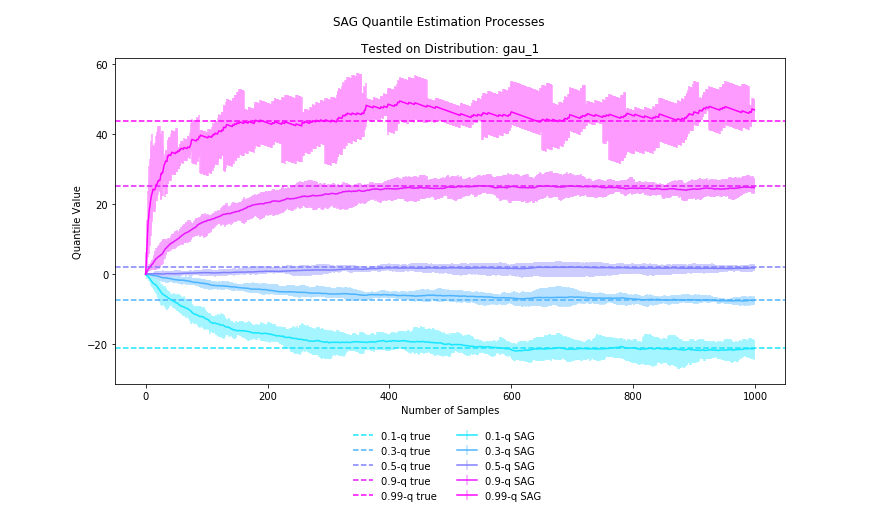
\includegraphics[width=1\columnwidth]{distro/gau_1_proc.png}
    \caption{SAG Process from \textit{gau-1} Distribution}
    \label{fig: sag_proc}
\end{figure}

\begin{figure}[H]
    \centering
	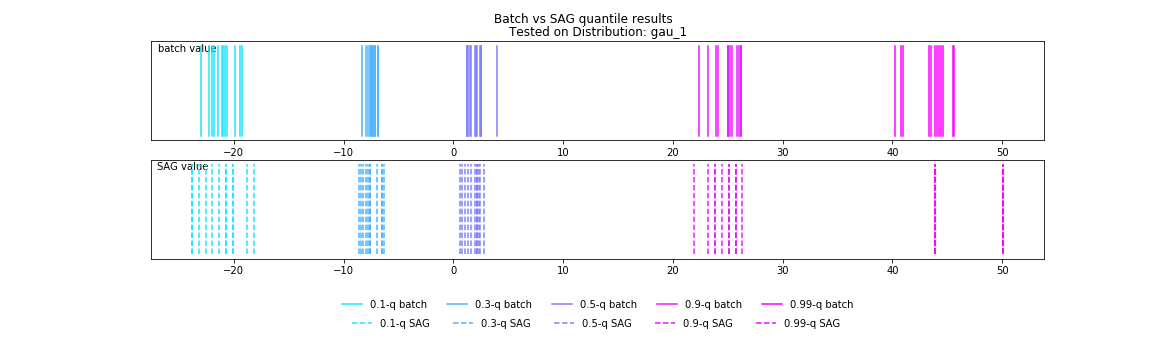
\includegraphics[width=1\columnwidth]{distro/gau_1_res.png}
    \caption{SAG Result from \textit{gau-1} Distribution}
    \label{fig: sag_res}
\end{figure}

\begin{figure}[H]
    \centering
	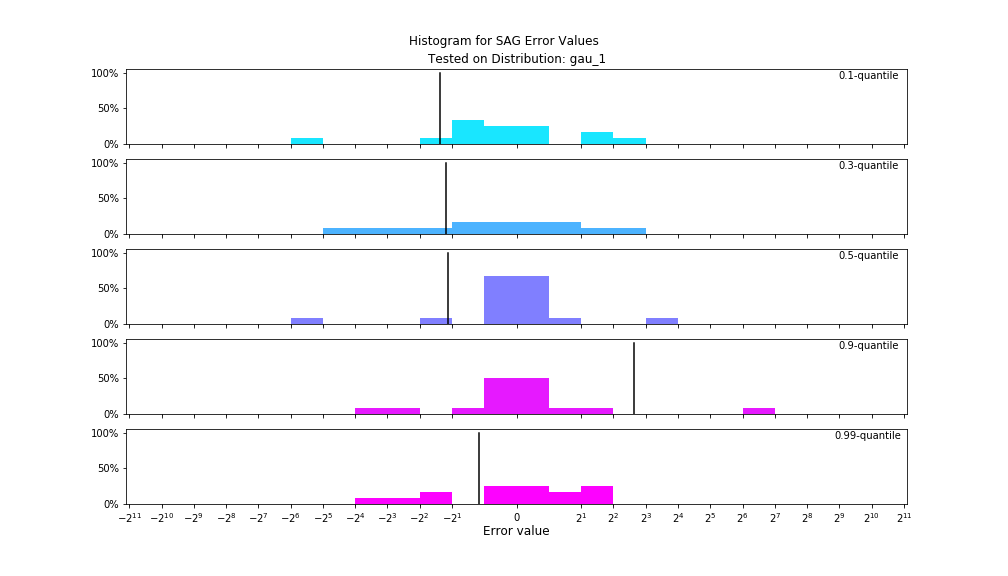
\includegraphics[width=1\columnwidth]{distro/gau_1_err.png}
    \caption{SAG Error from \textit{gau-1} Distribution}
    \label{fig: sag_err}

\end{figure}


\subsection{Smooth Functions}
\label{subsec: smooth_func}
The pinball loss function we use for the SGD quantile estimation is convex but not smooth. 
Theoretically, however, both SGD and SAG methods need smoothness for the guarantee of convergence. Although the practical experiments have shown that there is evidence of convergence in final performance, it remains a serious problem for our SGD quantile estimation methods. In this section, we present the analysis on the non-smoothness problem, followed by the potential solutions and further discussions on them.

\subsubsection{The Pinball Loss Functions}
\graphicspath{{Figures/Stepsize_adapt/Smooth_func/}{./}} 

The pinball loss function evaluates the loss from a data point $x$ for estimation of the $\tau$-quantile.

\textbf{quote the equation of pinball loss function and it's derivative}

The fact that the pinball loss function is not differentiable at $x= 0$ has became a problem for the stochastic gradient descent which uses derivatives of object functions.

\begin{figure*}[h!]
	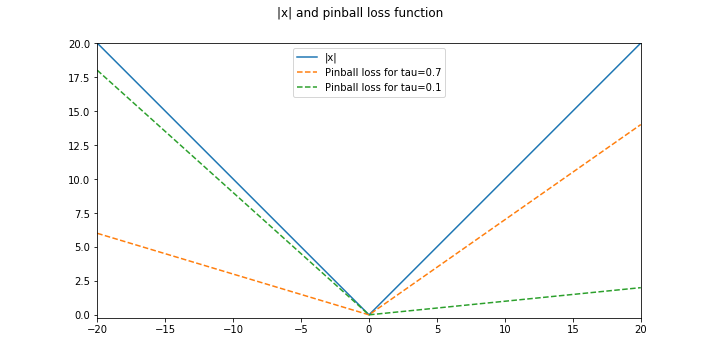
\includegraphics[width=1\columnwidth]{abs_pinball.png}
	\caption{Comparison between $|x|$ and the pinball loss function with different $\tau$ values}
\end{figure*}

The absolute function and the pinball loss function are obviously very much alike. In fact, with simple manipulation, the pinball loss function can be written in the form of absolute function as 
\begin{equation}
    l_\tau(x) = 
    \begin{cases}
        \tau \cdot |x| & {x \geq 0} \\
        (1-\tau) \cdot |x| & \text{otherwise}
    \end{cases}
\end{equation}
The pinball loss function is the combination of $|x|$ on the two parts $x<0$ and $x>0$ with different constant scale. 
If the derivative of the smooth function for $|x|$ at $x=0$ is $0$, we can also use the same approximation function respectively for the two parts of the pinball loss.
\\\\
In section \ref{subsec: smooth_sqrt} and \ref{subsec: smooth_new}, we show two approximation functions with regards to the absolute function $f = |x|$, along with the application of the approximations on the pinball loss function.

\subsubsection{Smooth function 1: a simple approxitmation}
\label{subsec: smooth_sqrt}

For $f = |x|$, a common and simple smooth approximation is $
    f = \sqrt{x^2 + \mu^2}
$.
 The convergence towards the absolute function is then proved by \citeauthor{voroninConvolutionBasedSmooth2015a}\cite{voroninConvolutionBasedSmooth2015a} that 
\begin{equation}
    ||x| - \sqrt{x^2 + \mu^2}| \leq \mu \text{  where } \mu > 0 \in \mathbb{R}
\end{equation}
\\
The smooth function application on the pinball loss function is:
\begin{equation}
    l_\tau(x) \approx 
    \begin{cases}
        \tau \cdot \sqrt{x^2 + \mu^2} & {x \geq 0} \\
        (1-\tau) \cdot \sqrt{x^2 + \mu^2} & {x < 0}
    \end{cases}
\end{equation}
and the derivative is
\begin{equation}
    l_\tau\prime(x) \approx 
    \begin{cases}
        \tau \cdot \frac{x}{\sqrt{x^2 + \mu^2}} & {x > 0} \\
        0 & {x=0} \\
        (1-\tau) \cdot \frac{x}{\sqrt{x^2 + \mu^2}} & {x<0}
    \end{cases}
\end{equation}
\subsubsection{Smooth function 2: a transcendental approximation}
\label{subsec: smooth_new}

For a better approximation accuracy, \citeauthor{bagulSMOOTHTRANSCENDENTALAPPROXIMATION2017}\cite{bagulSMOOTHTRANSCENDENTALAPPROXIMATION2017} proposes a new transcendental approximation function 
 \begin{equation}
    g(x) = x \cdot \tanh(x/\mu) \text{  where } \mu > 0 \in \mathbb{R}
 \end{equation}
which also satisfies
\begin{equation}
    ||x| - x \cdot tanh(\frac{x}{\mu})| < \mu
\end{equation}
The derivative of the approximation is
\begin{equation}
    \frac{dg(x)}{dx} = \frac{x}{\mu} \cdot sech^2 (\frac{x}{\mu}) + tanh(\frac{x}{\mu})
\end{equation}
For the pinball loss function, we now have its smooth function in the form:
\begin{equation}
    l_\tau(x) \approx 
    \begin{cases}
        \tau \cdot x \cdot \tanh(x/\mu) & {x\geq 0}\\
        (1-\tau) \cdot x \cdot \tanh(x/\mu) & {x < 0}
    \end{cases}
\end{equation}
and the derivative is
\begin{equation}
\label{eq:smooth_new_d}
    l_\tau\prime(x) \approx 
    \begin{cases}
        \tau \cdot \frac{x}{\mu} \cdot sech^2 (\frac{x}{\mu}) + tanh(\frac{x}{\mu}) & {x\geq 0}\\
        0 & {x=0}\\
        (1-\tau) \cdot \frac{x}{\mu} \cdot sech^2 (\frac{x}{\mu}) + tanh(\frac{x}{\mu}) & {x < 0}
    \end{cases}
\end{equation}
\subsubsection{Discussion and Conclusion}

In this part, we will compare the two alternative smooth functions in the following aspects: computer efficiency, approximation accuracy and
convexity. 
\begin{itemize}
    \item Computation efficiency: \\
    It is proved by \citeauthor{ramirezX2MostComputationally2014}\cite{ramirezX2MostComputationally2014} that $f = \sqrt{x^2 + \mu^2}$ is the most computationally efficient smooth approximation to $|x|$.
    
    On the other hand, we can see from equation \ref{eq:smooth_new_d}, the derivative for $g(x) = x \cdot \tanh(x/\mu)$ is more difficult to compute.
    \item Approximation accuracy: \\
    The following plots show intuitively how fast the two smooth functions approach to $|x|$ for $\mu = 0.01$ and $\mu = 0.001$.
    
    \begin{figure*}[h!]
        \includegraphics[width=1\columnwidth]{{mu_0.001}.png}
        \caption{Comparison between the two smooth functions when $\mu = 0.001$}
    \end{figure*}

    \begin{figure*}[h!]
        \includegraphics[width=1\columnwidth]{{mu_0.0001}.png}
        \caption{Comparison between the two smooth functions when $\mu = 0.0001$}
    \end{figure*}

    We can see $ x \cdot \tanh(x/\mu)$ has a better accuracy.

    \item Convexity\\
    $f = \sqrt{x^2 + \mu^2}$ is convex and  $g(x) = x \cdot \tanh(x/\mu)$ is not.
\end{itemize}

The form of smooth function \text{does not really matter for SAG}. It is important to know the existence of Lipschitz continuous smooth function, and then the $L$ of such function must satisfy
\begin{equation}
    L \leq min(|\tau|, |1-\tau|)
\end{equation}
So that no matter which smooth function is used, we can simply take $min(|\tau|, |1-\tau|)$ to compute the step size $\alpha$ for SAG. However, we can still implement those smooth functions for SGD. Further researches can be done on different smooth function implementation on SGD.

\section{Doubling and Halving SGD (DH-SGD)}
\label{sec: DH_SGD}

Although SAG has a faster convergence rate than SGD, it is clear that the fluctuation problem after convergence still exists. Is it possible that a step size adaptation of SGD can minify the fluctuation after the convergence, and at the same time have an improved convergence rate? In this section, we propose a simple algorithm called Doubling and Halving Stochastic Gradient Descent (DH-SGD), which empirically improve those two problems.

\subsection{Method Description}

The idea of the DH-SGD method is trivial - increase the step size if it is too big, and decrease the step size if it is too small. We choose the change of step sizes to be exponential, specifically, increasing it to double size or decrease it to half size. However, the standard on the scale of step size can be vague. 

Here we use an intuitive idea which tracks the proportion of increase and decrease updates among an interval of updates. For example, for every 200 epochs, the proportion of increase updates is $P^+$, and that of decrease update is $P^-$, we compute $P = P^+ - P^-$ as the difference between the proportional difference between two update directions. If $P$ is too far from the ideal value $P^*$ ($\mathbb{E}(P)$ for converged quantile estimate), then it means the updates are mostly in one direction, which is likely caused by the trend towards convergence, meaning that the step size is too small. Otherwise if $P$ is too close to $P^*$, we believe it is the signal that the convergence has already been reached, and now it is time to reduce the step size for a smaller fluctuation. 

According to the SGD update, the current quantile estimate decrease when it sees an data point smaller than it, and increases on seeing a smaller one.
It means when the quantile estimate for $\tau$-quantile has converged, the proportion of increase update $P^+_\tau$ should be the proportion of data points bigger than it, which is $1-\tau$. Similarly, we have the corresponding expectation that $P^-_\tau = \tau$.
Thus we have the ideal value for quantile probability $\tau$ defined as
\begin{equation}
    P^*_\tau = \mathbb{E}(P_\tau) = \mathbb{E}(P^+_\tau) - \mathbb{E}(P^-_\tau) = (1-\tau) - \tau = 1 - 2\tau \in (-1, 1)
\end{equation}
We use Euclidean distance to measure how close $P_\tau$ is to $P_\tau^*$. If $P_\tau \in (P^*_\tau- 0.01, P^*_\tau+ 0.01)$, it means they are too close and the step size is too big. And if $P_\tau \not\in (P^*_\tau- 0.1, P^*_\tau+ 0.1)$, it means they are too faraway and the step size is too small. 
The psedu-code of DH-SGD is shown as algorithm~\ref{alg:DH_SGD} :

% \marginpar{THe step size scaler is different for different quantiles}
\begin{algorithm}
    \caption{DH-SGD algorithm}\label{alg:DH_SGD}
    \begin{algorithmic}[1]
        \Require{Data Stream $X$, $\tau$, $1$ unit of memory $q$, epoch check size $c$}
        \Ensure{$q$}
        % \Procedure{frugal}{$X,\tau$}            \Comment{X is the dataset}
        \State{idealProportion $p = 1- 2\tau$}
        \State{epochCount $ec = 0$}                       \Comment{The counter for epochs}
        \State{directionCount $dc = 0$}                   \Comment{The accumulation of directions}
        \State{scaler $s = 1$}                    \Comment{The scaler for step size}
        \State {Initialize} $q$                 \Comment{Default initialization $q_0$ = 0}
        \State{}
            \For{$x_i$ in $X$}                  \Comment{Parameter update for each input data point}
                \State{}
                \State{$ec = ec+ 1$}   
                \If{$ec$ \textit{mod} $c = 0$}            \Comment{Change scaler for every $c$ epochs}
                    \If{$\frac{dc}{c} \in (p-0.01, p+0.01) $ }               
                        \State{$s = 2s$}               \Comment{Double $s$ if the update is mostly in one direction}         
                    \Else {\textbf{if} $\frac{dc}{c} \not\in (p-0.1, p+0.1)$ \textbf{then}}  
                        \State{$s = 0.5s$}             \Comment{Halve $s$ if the update direction barely changes}
                    \EndIf
                
                \EndIf
                \State{}
                \State{\textbf{set} $\alpha_i = 1$}             \Comment{$\alpha_i$ can use other settings}
                \State{$\alpha_i = \alpha_i \cdot s$}        \Comment{Scale original step size with $s$}
                \If{$x_i > q$}                  
                    \State{$q = q + \alpha_i \tau$}
                    \State{$dc = dc + 1$}                   \Comment{Direction count $+1$ if updated upwards}
                \Else {\textbf{if} $x_i < q$ \textbf{then}}                     
                    \State{$q = q - \alpha_i (1-\tau)$}
                    \State{$dc = dc -1$}                    \Comment{Direction count $-1$ if updated downwards}

                \EndIf
            \EndFor
        \State{}
        \State \textbf{return} $q$
        % \EndProcedure
    \end{algorithmic}
\end{algorithm}

\subsection{Experiments}
\graphicspath{{Figures/Stepsize_adapt/Adaptive_stepsize/}{./}} 
\label{subsec: DB_SGD_exp}
As the 
Again we test the DH-SGD on the data stream of size 1000 of \textit{gau-1} distribution. The experiment results are shown in figure~\ref{fig: DH_SGD_proc}, \ref{fig: DH_SGD_res} and \ref{fig: DH_SGD_err}.
Interesting Observations:
\begin{enumerate}
    \item The change of step size has a very obvious improvement on convergence rate. From figure~\ref{fig: DH_SGD_proc}  we can see all the quantiles has their convergence rate at the same or faster rate compared with SGD. For example, both $0.99$ and $0.9$-q DH-SGD have a doubled step size at epoch 200, and the former reaches its convergence around epoch 900 (compared with more than 1000 in SGD) and the latter reaches convergence within 300 epochs (compared with around 600 in SGD). The other three quantiles have basically the same convergence rate.
    
    \item The fluctuation after convergence are also improved overall. All the quantiles except for the $0.1$-q DH-SGD has a denser results distribution around the batch results (figure~\ref{fig: DH_SGD_res}). However, there are also results that stand outs from nearly every estimation distribution, which means the reduce of fluctuation is not stable.
    
    \item The affect on error value is a combined result from denser distribution of accurate results and more not-accurate results. Take the $0.99$-q DH-SGD in figure~\ref{fig: DH_SGD_err} for example, although most of the errors values are within the range ($-2^0, 2^2$), the existence of two bigger similarity values at $(-2^6, -2^5)$ and $(-2^4, -2^3)$ drag the mean error value further away from $0$. It is fair to argue the estimation error is still within the accuracy requirement range, but it is worse compared with the result in SGD, where the $0.99$-q SGD does not even converge. Although the fluctuation has been decreased by DH-SGD (figure~\ref{fig: DH_SGD_res}), the overall error values are also effected by only a small amount of estimations with bigger fluctuation. 
\end{enumerate}

\begin{figure}[H]
    \centering
	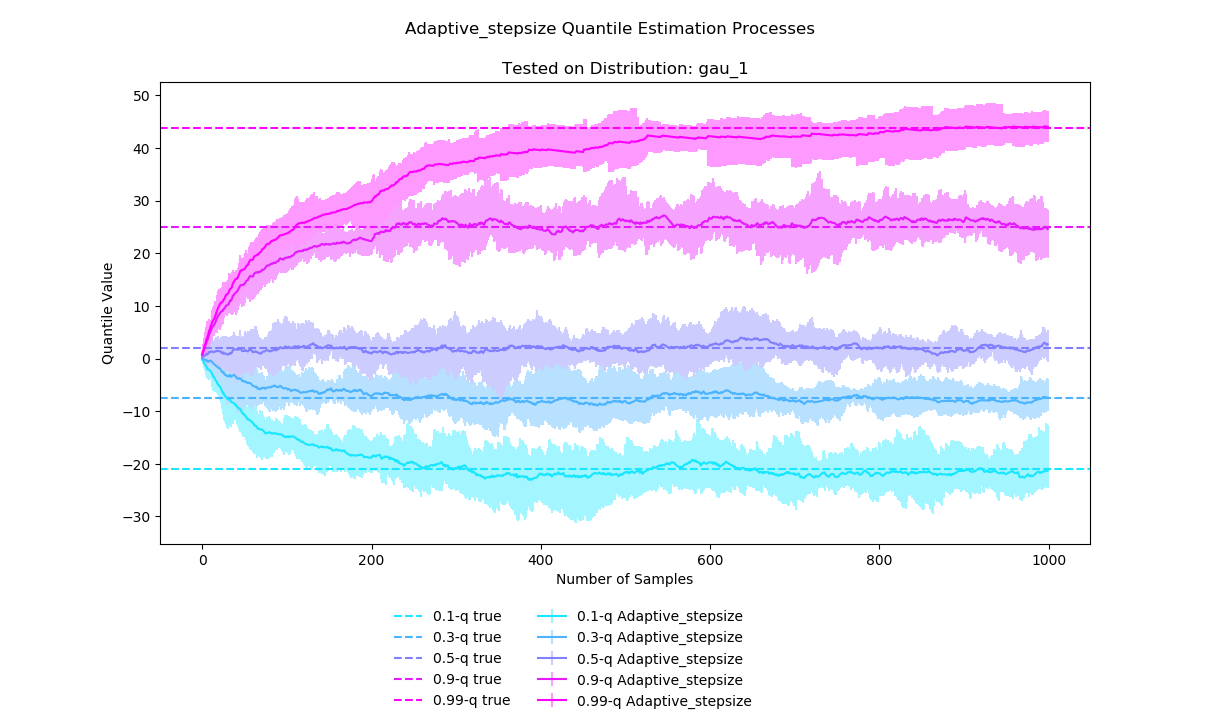
\includegraphics[width=1\columnwidth]{distro/gau_1_proc.png}
    \caption{DH-SGD Process from \textit{gau-1} Distribution}
    \label{fig: DH_SGD_proc}
\end{figure}


\begin{figure}[H]
    \centering
	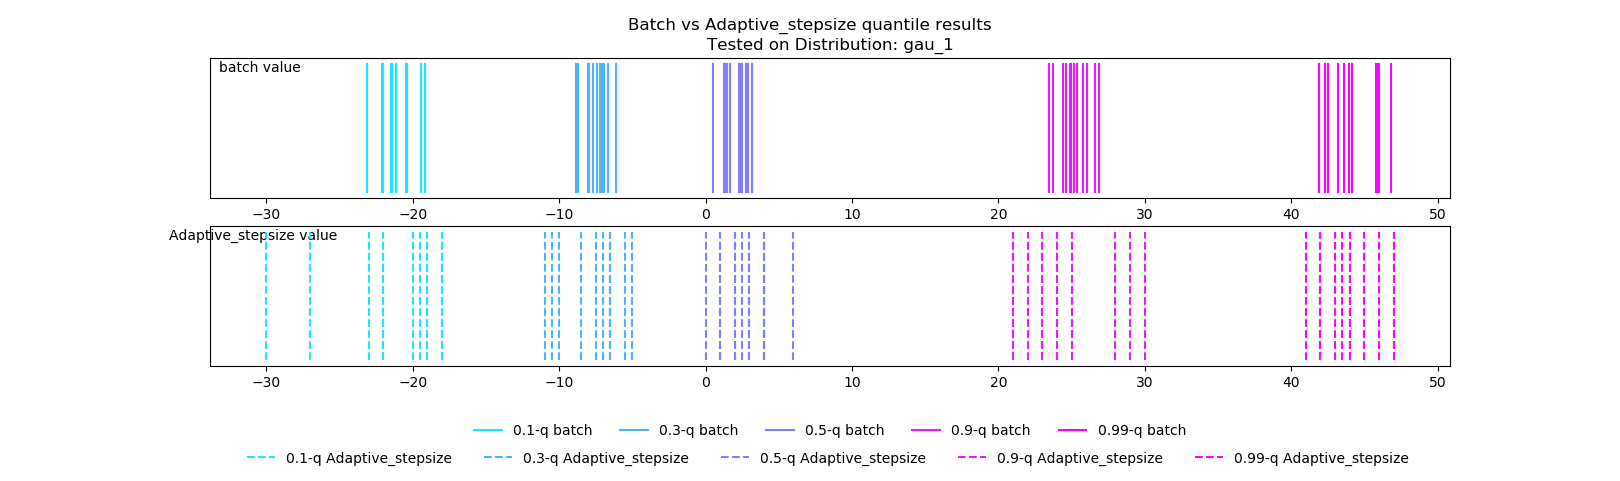
\includegraphics[width=1\columnwidth]{distro/gau_1_res.png}
    \caption{DH-SGD Results from  \textit{gau-1} Distribution}
    \label{fig: DH_SGD_res}

\end{figure}

\begin{figure}[H]
    \centering
	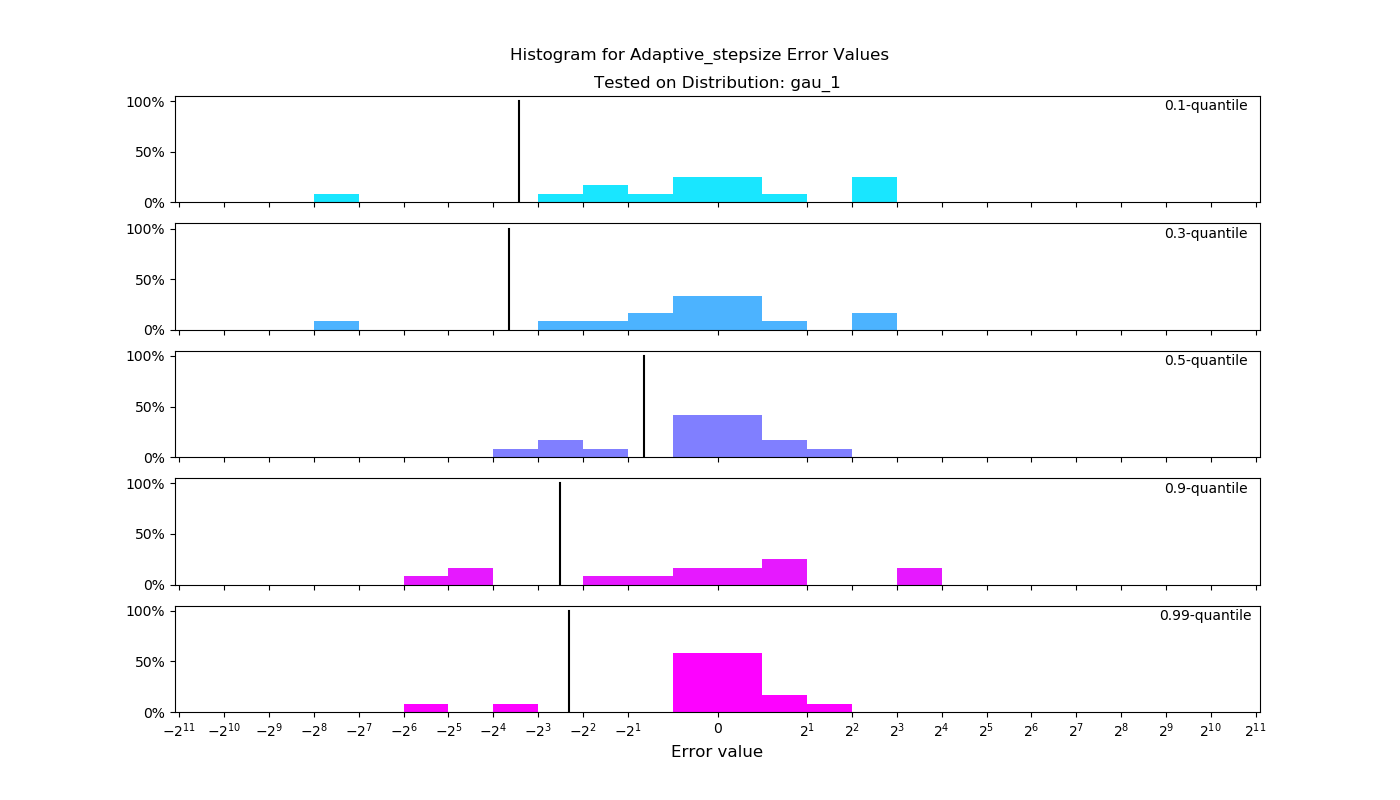
\includegraphics[width=1\columnwidth]{distro/gau_1_err.png}
    \caption{DH-SGD Error from \textit{gau-1} Distribution}
    \label{fig: DH_SGD_err}

\end{figure}

\subsection{Improvements on DH-SGD}

The small amount of estimations with fluctuation problems is a signal that the current standards for step size adaptation needs improvements. There are two potential ways for the improvements.

The first one is to change the epoch check size $c$, which determines how often to change the step size during the estimation. As the size and distribution of data stream is unknown, it is possible for the pre-defined parameter to be either too small or too big. If $c$ is small, it is more likely to have the recent $c$ updates to reach an extreme amount which leads to a step size change which should have been the other way around. For example, if $c = 3$, it is likely that all the recent $3$ updates are in the same direction even when the estimation has converged. In this case the step size is doubled when it should have been halved. On the other hand, if $c$ is big, for example, 100000, then it takes much longer for the convergence acceleration to happen. However, we cannot know beforehand which setting is more suitable for the unknown data stream. In this situation, the choice of epoch check size is hard to be improved.

The second one is about the standards on how close is $P_\tau$  from $P_\tau^*$. The current measurement takes the same value for all $\tau \in (0,1)$, while a more accurate distant can be calculated from quantile probability $\tau$ and epoch check size $c$. Specifically, one SGD update has only two options: increase or decrease(we ignore the keep same because the possibility is $0$). Ideally if the quantile has already reached the convergence, their possibilities are $1-\tau$ and $\tau$. The possibility of having $x$ increase updates from the dataset of size $c$ is now a binomial distribution problem, where the success probability $b = 1-\tau$.
Generally, the possibility of having exactly $x$ successes with possibility $b$ from $n$ trials is:
\begin{equation}
    F(x ; n,b)=\sum_{i=0}^{ x\rfloor}\left(\begin{array}{c}
    n \\
    i
\end{array}\right) b^{i}(1-b)^{n-i}
\end{equation}
And the distribution of the binomial possibilities are shown in figure~\ref{fig: binomial}
\begin{figure}[H]
    \centering
	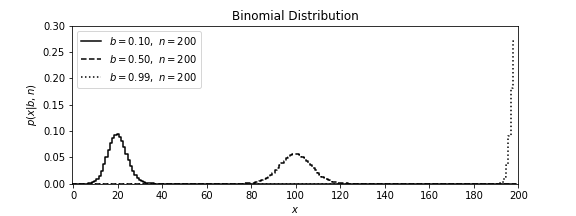
\includegraphics[width=1\columnwidth]{Binomial.png}
    \caption{DH-SGD Error from \textit{gau-1} Distribution}
    \label{fig: binomial}
\end{figure}
As shown in the plot, the distribution of number of successful trails are different and are depended on the success possibilities. It means the same distance standard for different $\tau$-quantiles has a different effect. We can improve this by computing the increase update distribution of each quantile and derive their distance standards respectively. Since it is only a discussion of improvement ideas, the details of the implementation is not included here.

\section{Conclusion}
\label{sec: stepsize_adaptation_conclusion}

To sum up, SAG and DH-SGD both improve the convergence rate of SGD. SAG improves the complexity of convergence rate in theory, but might empirically slows down the convergence when the step size scaler is smaller that the SGD default step size $1$ and the convergence of SGD is already fast. The DH-SGD algorithm, on the other hand, has illustrated obvious convergence improvements on all quantiles in experiments while its convergence can not be guaranteed.

The fluctuation rate after convergence, however, is solved by neither algorithm. The step size scaler of SAG stays consistent for any updates, so the fluctuation is not improved. DH-SGD changes the step sizes after regularly but cannot prevent the inaccurate estimation caused by non-convergence problem. A potential research direction is to improve the fluctuation and convergence problem by a combination of SAG and DH-SGD.

